\documentclass[11pt,a4paper]{article}
\usepackage[hyperref]{emnlp2020}
\usepackage{times}
\usepackage{latexsym}
\usepackage{tabularx}
\usepackage{graphicx}
\usepackage{float}
\usepackage{enumerate}
\usepackage{amssymb,amsmath}
\usepackage{color}
\usepackage{bm}
\usepackage{makecell}
\usepackage{multi row}
\usepackage{array}
\usepackage{resizegather}
\usepackage{refcount}
\usepackage{fixfoot}
\usepackage{hyperref}
\usepackage{url}
\usepackage{subcaption}  
\usepackage{bbm}
\renewcommand{\UrlFont}{\ttfamily\small}
\usepackage{algorithm}
\usepackage{algorithmicx}
\usepackage{algpseudocode}

\usepackage{microtype}

% comments
\newif\ifcomment
\commenttrue
%\commentfalse
\ifcomment
\newcommand{\kc}[1]{\textcolor{red}{KC: #1}}
\newcommand{\tl}[1]{\textcolor{blue}{TL: #1}}
\newcommand{\ql}[1]{\textcolor{cyan}{QL: #1}}
\newcommand{\cm}[1]{\textcolor{orange}{CM: #1}}
% Chris' marginal notes
\definecolor{CMpurple}{rgb}{0.6,0.18,0.64}
\newcommand\cmm[1]{\marginpar{\tiny\raggedright\textcolor{CMpurple}{\textsf{\bfseries CM\@: #1}}}}
\else
\newcommand{\kc}[1]{}
\newcommand{\tl}[1]{}
\newcommand{\ql}[1]{}
\newcommand{\cm}[1]{}
\newcommand{\cmm}[1]{}
\fi

% Pretty tables
\newcommand\tstrut{\rule{0pt}{2.6ex}}         
\newcommand\bstrut{\rule[-1.0ex]{0pt}{0pt}}   
\newcommand{\thinline}{\Xhline{1.5\arrayrulewidth}}
\newcommand{\thickline}{\Xhline{2.5\arrayrulewidth}}
\newcommand{\tsep}	{\bstrut \\ \thinline}
\newcommand{\tsept}	{\bstrut \\ \thickline}
\newcommand{\ttop}{\thickline}
\newcommand{\tbottom}{\bstrut \\ \thickline}
\newcommand{\replace}[3] {
    \textsc{replace}(#1, #2, #3)
    %#1_{#3 \backslash #2}
}

% Mini headers
\newcommand{\xhdr}[1]{\vspace{0mm}\noindent{{\bf #1}}\hspace{1.3mm}}

% Shortcuts
\newcommand{\aln}[1] {
	\begin{align} #1 \end{align}
}
\newcommand{\alns}[1] {
	\begin{align*} #1 \end{align*}
}
\newcommand{\bmx}{\bm{x}^\text{masked}}
\newcommand{\bfx}{\bm{x}^\text{noised}}
\newcommand{\lossmle}{\mathcal{L}_{\text{MLE}}(\theta)}
\newcommand{\lossmlm}{\mathcal{L}_{\text{MLM}}(\theta)}
\newcommand{\lossnce}{\mathcal{L}_{\text{NCE}}(\theta)}
\newcommand{\lossq}{\mathcal{L}_{\text{noise}}(\theta_q)}
\newcommand{\losspsce}{\mathcal{L}_{\text{PSCE}}(\theta_q)}
\newcommand{\Z}{Z_\theta(\cntxt)}
\newcommand{\I}{\bm{m}}
\newcommand{\bx}{\bm{x}}
\newcommand{\bw}{\bm{w}}
\newcommand{\bh}{\bm{h}}
\newcommand{\cntxt}{\bx_{\backslash t}}
%\newcommand{\cntxt}{\bx_{\bar{t}}}
\newcommand{\vocab}{\mathcal{V}}
\newcommand{\up}{\hat{p}_\theta}
\newcommand{\pdata}{p_\text{data}}
\newcommand{\E} {\mathop{\mathbb{E}}}
\newcommand{\hbx}{\hat{\bm{x}}}
\newcommand{\mask}{\texttt{[MASK]}}
\newcommand{\hf} { \overrightarrow{\bh} }
\newcommand{\hb} { \overleftarrow{\bh} }
\newcommand{\bs} {\bm{s}}
\DeclareMathOperator*{\argmax}{arg\,max}

\usepackage{etoolbox}
\newcommand{\zerodisplayskips}{
\addtolength{\abovedisplayskip}{-1pt} %try 2pt
\addtolength{\belowdisplayskip}{-1pt}
\addtolength{\abovedisplayshortskip}{-1pt}
\addtolength{\belowdisplayshortskip}{-1pt}
}
\appto{\normalsize}{\zerodisplayskips}
\appto{\small}{\zerodisplayskips}
\appto{\footnotesize}{\zerodisplayskips}

\aclfinalcopy

\title{Pre-Training Transformers as Energy-Based Cloze Models}

% \author{First Author \\
%   Affiliation / Address line 1 \\
%   Affiliation / Address line 2 \\
%   Affiliation / Address line 3 \\
%   \texttt{email@domain} \\\And
%   Second Author \\
%   Affiliation / Address line 1 \\
%   Affiliation / Address line 2 \\
%   Affiliation / Address line 3 \\
%   \texttt{email@domain} \\}

\author{Kevin Clark$^1$ \hspace{3mm} Minh-Thang Luong$^2$ \hspace{3mm} Quoc V. Le$^2$ \hspace{3mm} Christopher D. Manning$^1$\\
   $^1$Stanford University \hspace{6mm} $^2$Google Brain \\
   {\tt kevclark@cs.stanford.edu, thangluong@google.com} \\
   {\tt qvl@google.com, manning@cs.stanford.edu} \\
 }
 
\date{}

% Footnote about treating correct replacements as originals

\begin{document}
\maketitle
\begin{abstract}
% Masked language model pre-training is highly successful in NLP.
% %and energy-based models have proven effective at various generative tasks.
% Meanwhile, in other contexts energy-based models have proven effective at various generative tasks.
% Putting the two together, we introduce Electric, an energy-based masked language model for representation learning over text.
% Like BERT, it is a conditional generative model of tokens given their surrounding contexts. 
% %However, given a context, the network scores only a single candidate token rather than producing a full distribution over possible tokens. 
% However, Electric does not explicitly mask text or use an output softmax; instead it directly produces an un-normalized probability for each input token.
% We train Electric with noise-contrastive estimation and elucidate how this learning objective is closely related to the recently proposed ELECTRA pre-training method. 
% Electric scores better than BERT when fine-tuned on downstream NLP tasks such as question answering and can efficiently perform better re-scoring of speech recognition n-best lists than conventional LMs.
% %produce pseudo-log-likelihood scores for text, which can be used in applications such as speech recognition. 
We introduce Electric, an energy-based cloze model for representation learning over text. 
Like BERT, it is a conditional generative model of tokens given their contexts. 
However, Electric does not use masking or output a full distribution over tokens that could occur in a context.
Instead, it assigns a scalar energy score to each input token indicating how likely it is given its context.
We train Electric using an algorithm based on noise-contrastive estimation and elucidate how this learning objective is closely related to the recently proposed ELECTRA pre-training method. %to assign low energies to data tokens and high energies to other ones
%Electric solves the pre-train/fine-tune discrepancy of MASK tokens in BERT and allows the candidate token and context to interact in the transformer layers instead of only in an output softmax. 
%Electric scores better than BERT but slightly worse than ELECTRA when fine-tuned on downstream NLP tasks. % such as question answering. 
%Furthermore, it can perform re-scoring of speech recognition n-best lists better than language models and faster than masked language models.
Electric performs well when transferred to downstream tasks and is particularly effective at producing likelihood scores for text: it re-ranks speech recognition n-best lists better than language models and much faster than masked language models. Furthermore, it offers a clearer and more principled view of what ELECTRA learns during pre-training.
\end{abstract}

\section{Introduction}

% Many recent language representation learning methods train a large neural network to predict the identity of a token conditioned on the context to its left (language models) or both sides (cloze models such as BERT \cite{devlin2018bert}).
% %Language models use the context to one side of the token while masked language models such as BERT \citep{devlin2018bert} use both sides.
% These existing methods follow the standard recipe of estimating token probabilities with an output softmax and using maximum-likelihood training, with other kinds of generative models remaining unexplored.  

% We instead train an Energy-Based Model (EBM) called Electric\footnote{Code will be released at \url{https://github.com/google-research/electra}} to perform the cloze task.
% %and show that it outperforms BERT \citep{devlin2018bert} across a range of transfer learning tasks. 
% %use generative pre-training tasks. For example, masked language models such as BERT \cite{devlin2018bert} generate tokens given their surrounding contexts.
% %These existing models follow the standard recipe of estimating token probabilities with an output softmax and using maximum-likelihood training, with other kinds of generative models remaining unexplored.  
% %We instead train an Energy-Based Model (EBM) called Electric\footnote{Code will be released at \url{http://anonymized}} to perform the masked language modeling task and show that it outperforms BERT.
% EBMs learn an energy function that assigns low energy values to inputs in the data distribution and high energy values to other inputs.  
% They are flexible because they do not have to compute normalized probabilities. 
% For example, Electric does not use masking or an output softmax, instead producing an energy score for each input token where a low energy indicates the token is likely.
% %Scoring every input is advantageous because it means Electric can re-rank the outputs of , while BERT requires running once with each token masked out.
% %We train Electric with noise-contrastive estimation \citep{Gutmann2010NoisecontrastiveEA}
% We propose a training algorithm for Electric that efficiently approximates a loss based on noise-contrastive estimation \citep{Gutmann2010NoisecontrastiveEA}. We then describe how the learning objective is closely related to the recently-proposed ELECTRA pre-training method \citep{clark2020electra}, providing a clearer picture of what ELECTRA learns. 
% %while on the surface ELECTRA appears quite different from BERT, this connection illustrates how they are %learning similar things.

% We evaluate Electric on GLUE \citep{wang2018glue} and SQuAD \citep{Rajpurkar2016SQuAD10}, where Electric substantially outperforms BERT but slightly under-performs ELECTRA.  
% However, a key advantage of Electric is its ability to efficiently produce pseudo-log-likelihood scores \citep{Salazar2019MaskedLM} for text: Electric is better at re-ranking the outputs of a speech recognition system than GPT-2 \citep{Radford2019LanguageMA} % because it is bidirectional 
% and is much faster at re-ranking than BERT because it scores all input tokens simultaneously rather than having to be run multiple times with different tokens masked out.
% % Electric is better at re-ranking the outputs of a speech recognition system than GPT-2 \citep{Radford2019LanguageMA} because it is bidirectional and is many times faster at re-ranking compared to BERT because it scores all input tokens in one passes rather than having to run once with each token masked out.
% Our results suggest that EBMs are a promising alternative to the standard generative models currently used for language representation learning.
% %\kc{More on re-ranking}

%\vspace{-3mm}

The cloze task \citep{Taylor1953ClozePA} of predicting the identity of a token given its surrounding context has proven highly effective for representation learning over text. BERT \citep{devlin2018bert} implements the cloze task by replacing input tokens with [MASK], but this approach incurs drawbacks in sample efficiency (only 15\% of tokens are masked out at a time) and introduces a pre-train/fine-tune mismatch where BERT sees [MASK] tokens in training but not in fine-tuning. 
ELECTRA \citep{clark2020electra} uses a new pre-training task that alleviates these disadvantages. Instead of masking tokens, ELECTRA replaces some input tokens with fakes sampled from a small generator network. The pre-training task is then to distinguish the original vs. replaced tokens. 
While on the surface it appears quite different from BERT, in this paper we elucidate a close connection between ELECTRA and cloze modeling.
In particular, we develop a new way of implementing the cloze task using an energy-based model (EBM).
Then we show the resulting model, which we call Electric, is closely related to ELECTRA, as well as being useful in its own right for some applications.\footnote{Code is available at \url{https://github.com/google-research/electra}}  

%First, we develop an energy-based (EBM) model we call Electric\footnote{Code will be released at \url{https://github.com/google-research/electra}} to perform the cloze task.
EBMs learn an energy function that assigns low energy values to inputs in the data distribution and high energy values to other inputs.  
They are flexible because they do not have to compute normalized probabilities. 
For example, Electric does not use masking or an output softmax, instead producing a scalar energy score for each token where a low energy indicates the token is likely given its context.
Unlike with BERT, these likelihood scores can be computed simultaneously for all input tokens rather than only for a small masked-out subset. 
We propose a training algorithm for Electric that efficiently approximates a loss based on noise-contrastive estimation \citep{Gutmann2010NoisecontrastiveEA}. 
Then we show that the training algorithm is closely related to ELECTRA; in fact, ELECTRA can be viewed as a variant of Electric using negative sampling instead of noise-contrastive estimation.


\begin{figure*}[tb]
\begin{center}
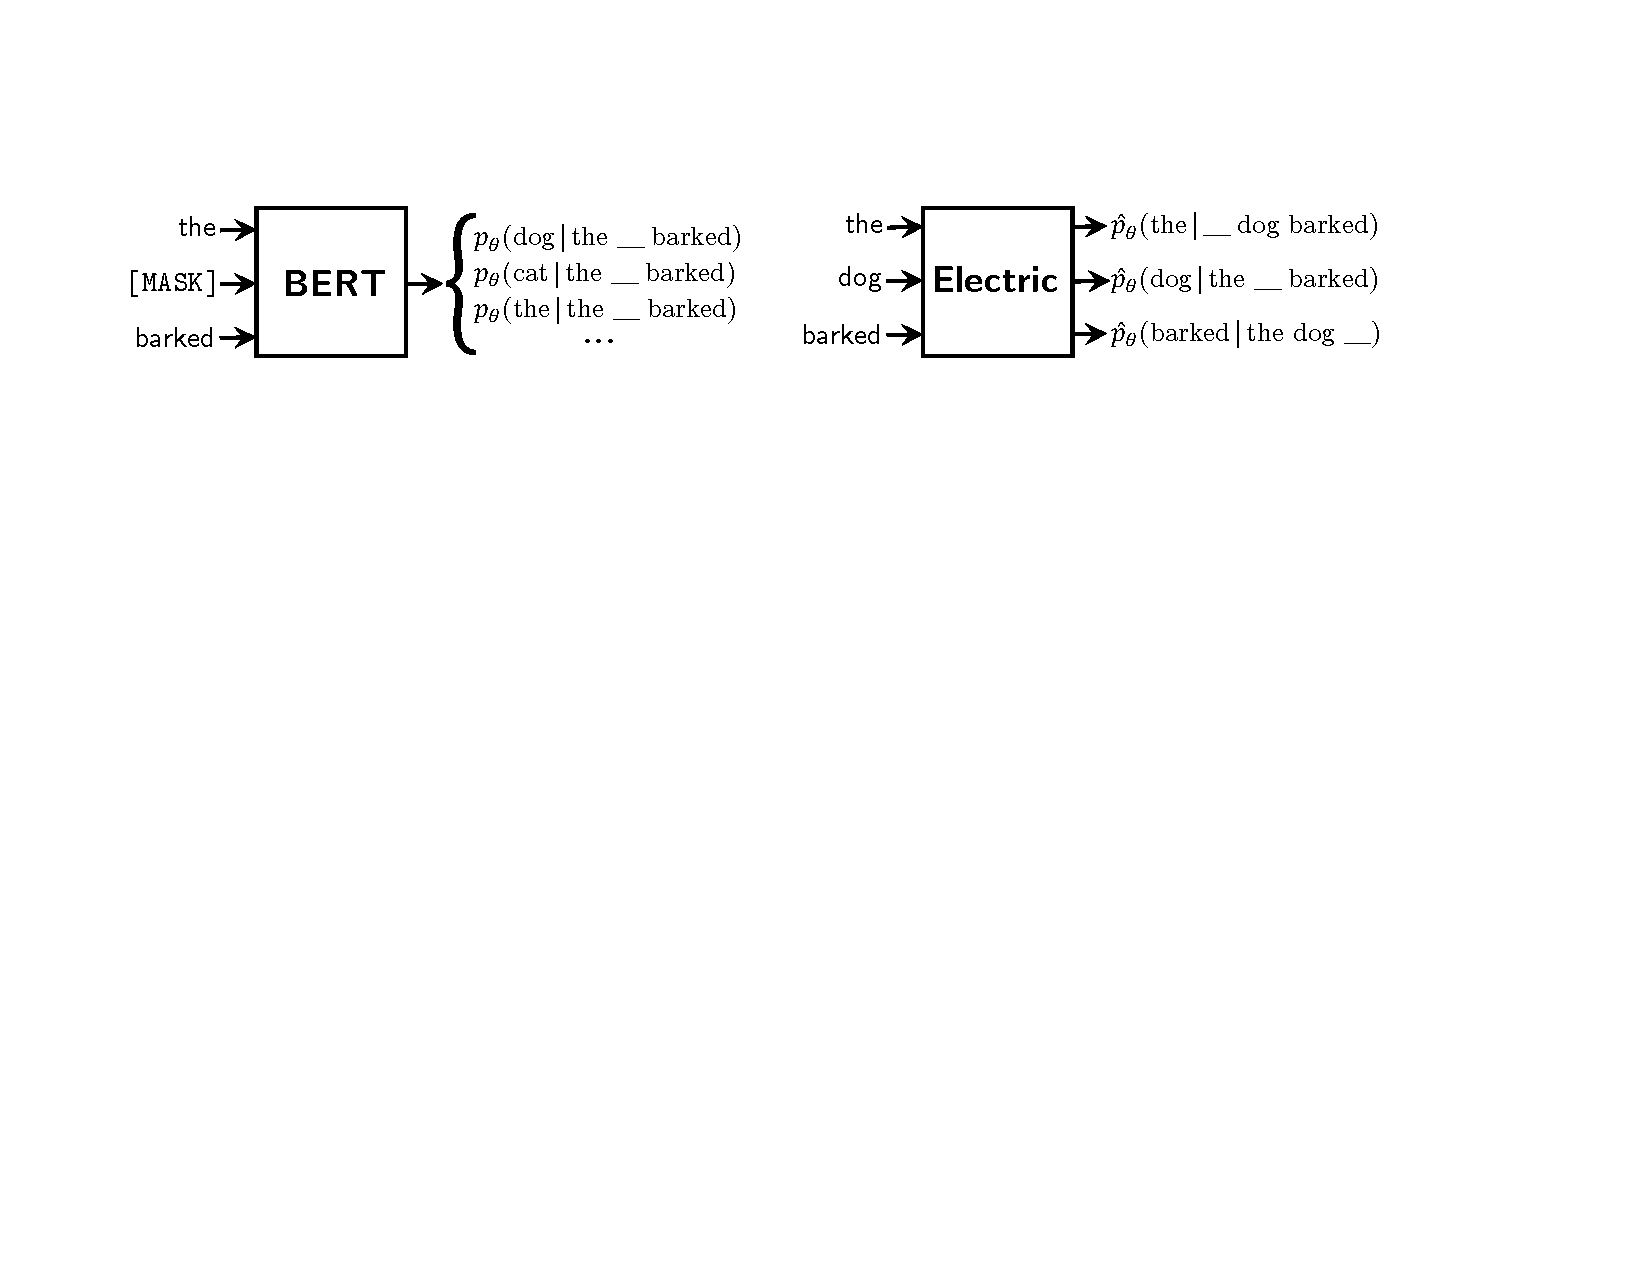
\includegraphics[width=1.0\textwidth]{fig/electric_cropped.pdf}
\end{center}
%\vspace{-1mm}
\caption{Comparison of BERT and Electric\@. Both model the probability of a token given its surrounding context, but BERT produces a full output distribution over tokens only for masked positions while Electric produces un-normalized probabilities (but no full distribution) for all input tokens.}
\vspace{-1mm}
\label{fig:overview}
\end{figure*}

We evaluate Electric on GLUE \citep{wang2018glue} and SQuAD \citep{Rajpurkar2016SQuAD10}, where Electric substantially outperforms BERT but slightly under-performs ELECTRA.  
However, Electric is particularly useful in its ability to efficiently produce pseudo-likelihood scores \citep{Salazar2019MaskedLM} for text: 
Electric is better at re-ranking the outputs of a speech recognition system than GPT-2 \citep{Radford2019LanguageMA} % because it is bidirectional 
and is much faster at re-ranking than BERT because it scores all input tokens simultaneously rather than having to be run multiple times with different tokens masked out.
In total, investigating Electric leads to a more principled understanding of ELECTRA and our results suggest that EBMs are a promising alternative to the standard generative models currently used for language representation learning.
%In total, our results suggest that EBMs are a promising alternative to the standard generative models currently used for language representation learning and our analysis offers more a principled understanding of ELECTRA. 




%train the model to generate a token given either the left or right context

%Intuition: recognizing a word as being correct is easier than generating the correct word from %scratch. 
%EBMs more flexible but harder to train because intractable density/partition function.
%ELECTRA performs much better than BERT and, on the surface, looks quite different.
%However, we show it is actually (implicitly) modeling the same thing.
%EBM perspective more principled leads to new ideas to improve performance.
%In particular we propose new noise network that is trained to match the EBM.
%Electric perfo\footnote{Code will be released at \url{http://anonymized}}.


\section{Method}


%\vspace{-1mm}

%\subsection{}

BERT and related pre-training methods \cite{baevski2019cloze, liu2019roberta,  lan2019albert}
train a large neural network to perform the cloze task.
These models learn the probability $\pdata(x_t | \cntxt)$ of a token $x_t$ occurring in the surrounding context $\cntxt = [x_1, ..., x_{t- 1}, x_{t+1}, ..., x_n]$.
Typically the context is represented as %$[x_1, ... , x_{t-1}, \mask, x_{t+1}, ... , x_n]$, 
the input sequence with $x_t$ replaced by a special \mask placeholder token. 
This masked sequence is encoded into vector representations by a transformer network \cite{Vaswani2017AttentionIA}.
Then the representation at position $t$ is passed into a softmax layer to produce a 
distribution over tokens $p_\theta(x_t | \cntxt)$ for the position.
%The negative log-likelihood loss for the model is
%over a dataset $\mathcal{D}$ of unlabeled text sequences of length $n$ is
%\aln{
% \lossmle = \frac{1}{|D|}\sum_{\bx \in \mathcal{D}} \frac{1}{n} \sum_{t=1}^n -\log(p_\theta(x_t | \cntxt))
%}
% \aln{
%     \lossmle = \E_{\substack{\bx \sim p_{\text{data}},\\ t \sim \text{unif}\{1, n\}}} -\log(p_\theta(x_t | \cntxt))
% }
%\kc{writing out equation for BERT's loss got a bit complicated, maybe I should just remove this?}
%However, to improve efficiency masked language models like BERT typically mask out $k$ tokens from each example rather than only one, giving the loss
%\aln{
  %\lossmlm = \frac{1}{|D|}\sum_{\bx \in \mathcal{D}} \frac{1}{\mathcal{|S|}} \sum_{\I \in \mathcal{S}} \frac{1}{k} \sum_{i=1}^k %-\log(p_\theta(x_{m_i} | \replace{\bx}{\I}{\mask}))
%}
% \aln{
% \lossmlm \E_{\bx, \I} \frac{1}{k} \sum_{i=1}^k -\log(p_\theta(x_{m_i} | \replace{\bx}{\I}{\mask}))
% }
%where $\mathcal{S} = \{\I: \I \subset [n] \land |\I| = k\}$ contains all possible selections of $k$ unique positions in the input sequence to mask out.
% where $\I$ is a set of $k$ positions in the input sequence sampled uniformly at random without replacement. 
% The loss in (2) is only equivalent to (1) if $-\log(p_\theta(x_t | \cntxt) = -\log(p_\theta(x_t | \replace{\bx}{\I}{\mask}))$, i.e., the additional masked-out tokens do not change the model's outputs. In practice, $k$ is set to a small value (for BERT, $k = \lceil0.15n\rceil$, i.e., 15\% of the tokens are masked out per example) to reduce this discrepancy.

\subsection{The Electric Model}

Electric also models $\pdata(x_t | \cntxt)$, but does not use masking or a softmax layer.
Electric first maps the unmasked input $\bx = [x_1, ..., x_n]$ into contextualized vector representations $\bh(\bx) = [\bh_1, ..., \bh_n]$ using a transformer network.
The model assigns a given position $t$ an energy score
\alns{
E(\bx)_t = \bw^T \bh(\bx)_t
}
using a learned weight vector $\bw$.
The energy function defines a distribution over the possible tokens at position $t$ as
\alns{
    p_\theta(x_t | \cntxt) &= \exp{(-E(\bx)_t)} / Z(\cntxt) \\
    &\hspace{-8mm} = \frac{\exp{(-E(\bx)_t)}}{\sum_{x' \in \vocab} \exp{(-E(\replace{\bx}{t}{x'})_t)}}
}
where $\replace{\bx}{t}{x'}$ denotes replacing the token at position $t$ with $x'$ and $\vocab$ is the vocabulary, in practice usually word pieces \cite{Sennrich2016NeuralMT}.
Unlike with BERT, which produces the probabilities for all possible tokens $x'$ using a softmax layer, a candidate $x'$ is passed in as {\it input} to the transformer. 
As a result, computing $p_\theta$ is prohibitively expensive because the partition function $\Z$ requires running the transformer $|\vocab|$ times.

\subsection{NCE Loss}
As computing the exact likelihood is intractable, training energy-based models such as Electric with standard maximum-likelihood estimation is not possible.
Instead, we use (conditional) Noise-Contrastive Estimation (NCE) \citep{Gutmann2010NoisecontrastiveEA, Ma2018NoiseCE}, which provides a way of efficiently training an un-normalized model that does not compute $\Z$.
NCE learns the parameters of a model by defining a binary classification task where samples from the data distribution have to be distinguished from samples generated by a noise distribution $q(x_t|\bx_{\backslash t})$. First, we define the un-normalized output
\vspace{-1mm}
\alns{
    \up(x_t | \cntxt) = \exp{(-E(\bx)_t)} 
}
\vspace{-1mm}
\noindent Operationally, NCE can be viewed as follows: \vspace{-1.2mm}
\begin{itemize}
    \item A positive data point is a text sequence $\bx$ from the data and position in the sequence $t$. \vspace{-1mm}
    \item A negative data point is the same except $x_t$, the token at position $t$, is replaced with a noise token $\hat{x}_t$ sampled from $q$. \vspace{-1mm}
    \item Define a binary classifier $D$ that estimates the probability of a data point being positive as\vspace{-1mm}
    \alns{\frac{n\cdot\up(x_t | \cntxt)}{n\cdot\up(x_t | \cntxt) + k\cdot q(x_t | \cntxt)}} \vspace{-5mm}
    \item The binary classifier is trained to distinguish positive vs negative data points, with $k$ negatives sampled for every $n$ positive data points. \vspace{-1mm}
\end{itemize}
\vspace{-1.2mm}
Formally, the NCE loss $\mathcal{L}(\theta)$ is
\alns{
%\mathcal{L}(\theta) &= \E_{\bx, t} \Biggl[-\log{\frac{\up(x_t | \cntxt)}{\up(x_t | \cntxt) + k\cdot q(x_t | \cntxt)}} + \\
%&k\cdot \E_{\hat{x}_t \sim q} \left[ -\log{\frac{k\cdot q(\hat{x}_t | \cntxt)}{\up(\hat{x}_t | \cntxt) + k\cdot q(\hat{x}_t | \bx_{\backslash t})}} \right] \Biggr]
n\cdot\E_{\bx, t} &\left[-\log{\frac{n \cdot \up(x_t | \cntxt)}{n \cdot \up(x_t | \cntxt) + k\cdot q(x_t | \cntxt)}} \right] + \\
k\cdot \hspace{-1.5mm} \E_{\substack{\bx, t \\ \hat{x}_t \sim q}} &\left[ -\log{\frac{k\cdot q(\hat{x}_t | \cntxt)}{n \cdot \up(\hat{x}_t | \cntxt) + k\cdot q(\hat{x}_t | \bx_{\backslash t})}} \right]
}

\noindent This loss is minimized when $\up$ matches the data distribution $p_\text{data}$ \cite{Gutmann2010NoisecontrastiveEA}.
A consequence of this property is that the model learns to be self-normalized such that $\Z = 1$. %The objective gives consistent parameter estimates provided the model has flexibility to be self-normalized for every context \cite{Ma2018NoiseCE}. 

\subsection{Training Algorithm}
To minimize the loss, the expectations could be approximated by sampling as shown in Algorithm~\ref{alg:naive}.
\begin{algorithm}
    \caption{Naive NCE loss estimation}
    \label{alg:naive}
    \begin{algorithmic}
    \State \textbf{Given:} Input sequence $\bx$, number of negative samples $k$, noise distribution $q$, model $\up$.
    %\State Using the binary classifier \\ $D(\bx)_t = -\log{\frac{n \cdot \up(x_t | \bx_{\backslash t})}{n*\up(x_t | \bx_{\backslash t}) + k\cdot q(x_t | \bx_{\backslash t})}}$
    \State \textbf{1.} Initialize the loss as \phantom{aaaaaaaaaaaaaaaa} $\sum_{t=1}^n \left( -\log{\frac{n \cdot \up(x_t | \bx_{\backslash t})}{n \cdot \up(x_t | \bx_{\backslash t}) + k\cdot q(x_t | \bx_{\backslash t})}} \right)$. 
    \State \textbf{2.} Sample $k$ negative samples according to $t \sim \text{unif}\{1, n\}$, $\hat{x}_t \sim q(x_t | \bx_{\backslash t})$. 
    \State \textbf{3.} For each negative sample, add to the loss $-\log{\frac{k \cdot q(\hat{x}_t | \bx_{\backslash t})}{n \cdot \up(\hat{x}_t | \bx_{\backslash t}) + k\cdot q(\hat{x}_t | \bx_{\backslash t})}}$.
    %\State where $\alpha = k / n$ is the ratio of noise to data samples.
    \end{algorithmic}
    \vspace{-1mm}
\end{algorithm}
%where $\alpha = k / n$ is the ratio of noise to data samples.
Taking the gradient of this estimated loss produces an unbiased estimate of $\nabla_\theta \mathcal{L}(\theta)$. 
However, this algorithm is computationally expensive to run, since it requires $k + 1$ forward passes through the transformer to compute the $\up$s (once for the positive samples and once for each negative sample). 
We propose a much more efficient approach that replaces $k$ input tokens with noise samples {\it simultaneously} shown in Algorithm~\ref{alg:efficient}. % where $\alpha = k / (n - k)$.
\begin{algorithm}
    \caption{Efficient NCE loss estimation}
    \label{alg:efficient}
    \begin{algorithmic}
    \State \textbf{Given:} Input sequence $\bx$, number of negative samples $k$, noise distribution $q$, model $\up$.  
    \State \textbf{1.} Pick $k$ unique random positions $R = \{r_1, ..., r_k\}$ where each $r_i$ is $1 \leq r_i \leq n$.
    \State \textbf{2.} Replace the $k$ random positions with negative samples: $\hat{x}_i \sim q(x_i | \bx_{\backslash i}) \text{ for } i \in R,$\\ $\bfx = \replace{\hbx}{R}{\hat{X}}$.
    \State \textbf{3.} For each position $t=1 \text{ to } n$: add to the loss
    $
    \begin{array}{l l}
    -\log{\frac{k \cdot q(\hat{x}_t | \bx_{\backslash t})}{(n - k)\cdot \up(\hat{x}_t | \bfx_{\backslash t}) + k\cdot q(\hat{x}_t | \bx_{\backslash t})}} & \text{if } t \in R\\
    -\log{\frac{(n - k)\cdot \up(x_t | \bfx_{\backslash t})}{(n - k)\cdot \up(x_t | \bfx_{\backslash t}) + k\cdot q(x_t | \bx_{\backslash t})}}              & \text{otherwise}
    \end{array}
    $
    %if $t \notin M$, 
    %$-\log{\frac{\up(x_t | \bfx_{\backslash t})}{\up(x_t | \bfx_{\backslash t}) + \alpha\cdot q(x_t | \bx_{\backslash t})}}$ to the loss. Otherwise add $-\log{\frac{\alpha \cdot q(\hat{x}_t | \bx_{\backslash t})}{\up(\hat{x}_t | \bfx_{\backslash t}) + \alpha\cdot q(\hat{x}_t | \bx_{\backslash t})}}$ to the loss.
    \end{algorithmic}
    \vspace{-1mm}
\end{algorithm}
It requires just one pass through the transformer for $k$ noise samples and $n - k$ data samples.
However, this procedure only truly minimizes $\mathcal{L}$ if $\up(x_t | \bx_{\backslash t}) = \up(x_t | \bx^{\text{noised}}_{\backslash t})$. To apply this efficiency trick we are making the assumption they are approximately equal, which we argue is reasonable because (1) we choose a small $k$ of $\lceil0.15n\rceil$ and (2) $q$ is trained to be close to the data distribution (see below). This efficiency trick is analogous to BERT masking out multiple tokens per input sequence. 

\subsection{Noise Distribution}
The noise distribution $q$ comes from a neural network trained to match $p_\text{data}$.
NCE commonly employs this idea to ensure the classification task is sufficiently challenging for the model \citep{Gutmann2010NoisecontrastiveEA,Wang2018LearningNT}. 
In particular, we use a two-tower cloze model as proposed by \citet{baevski2019cloze}, which is more accurate than a language model because it uses context to both sides of each token.
The model runs two transformers $T_{\textsc{ltr}}$ and $T_{\textsc{rtl}}$ over the input sequence. These transformers apply causal masking so one processes the sequence left-to-right and the other operates right-to-left.
The model's predictions come from a softmax layer applied to the concatenated states of the two transformers:
%\vspace{-5mm}
\alns{
    &\hf = T_{\textsc{ltr}}(\bx), \hspace{3mm} \hb = T_{\textsc{rtl}}(\bx) \\[-2pt]
    &\vspace{-15mm}q(x_t | \cntxt) = \text{softmax}(\bm{W} [\hf_{t - 1}, \hb_{t + 1}])_{x_t} 
}
\noindent The noise distribution is trained simultaneously with Electric using standard maximum likelihood estimation over the data.
The model producing the noise distribution is much smaller than Electric to reduce the computational overhead. 
%For a given input position, the model concatenates the previous left-to-right hidden state and next right-to-left hidden state.
%This representation is passed into a softmax layer to predict the token at the position.
%We use the two-tower model instead of a regular language model because it is more effective at modeling $p(x_t | \cntxt)$, having access to both the left and right context of $x_t$.


\subsection{Connection to ELECTRA}
Electric is closely related to the ELECTRA pre-training method. 
%Although we have presented Electric as though deriving it from scratch, Electric is very similar to the ELECTRA pre-training method. 
ELECTRA also trains a binary classifier (the ``discriminator") to distinguish data tokens from noise tokens (produced by a ``generator"). 
However, ELECTRA's classifier is simply a sigmoid layer on top of the transformer: ELECTRA models the probability of a token being negative (i.e., as replaced by a noise sample) as $\sigma(E(\bx)_t)$ where $\sigma$ denotes the sigmoid function.
Electric on the other hand models this probability as 
\alns{
&\frac{k \cdot q(x | \cntxt)}{n \cdot \exp{(-E(\bx)_t)} + k \cdot q(x | \cntxt)} =\\ &\sigma\left(E(\bx)_t + \log\left( \frac{k \cdot q(x | \cntxt)}{n} \right)\right)
}
While ELECTRA learns whether a token is more likely to come from the data distribution $\pdata$ or  noise distribution $q$, Electric only learns $\pdata$ because $q$ is passed into the model directly. This difference is analogous to using negative sampling \cite{Mikolov2013DistributedRO} vs. noise-contrastive estimation \cite{Mnih2013LearningWE} for learning word embeddings.

%An advantage of Electric over ELECTRA is that it provides (un-normalized) probabilities $\up$ for tokens, making it useful for applications such as re-ranking the outputs of text generation systems.\footnote{ELECTRA's binary classifier does score tokens, but we found these scores ineffective for re-ranking, see the appendix.} %because they measure if a token is more likely to come from the data or noise distribution, not the token's absolute likelihood.} speech recognition systems (see Section~\ref{sec:pll}). 
%While masked-language models such as BERT can also produce pseudo-log-likelihood, they require much more compute to do so.
A disadvantage of Electric over ELECTRA is that it is less flexible in the choice of noise distribution. Since ELECTRA's binary classifier does not need to access $q$, its $q$ only needs to be defined for negative sample positions in the input sequence. Therefore ELECTRA can use a masked language model rather than two-tower cloze model for $q$.
An advantage of Electric is that it directly provides (un-normalized) probabilities $\up$ for tokens, making it useful for applications such as re-ranking the outputs of text generation systems.
The differences between ELECTRA and Electric are summarized below. \\
% Electric is closely related to the ELECTRA pre-training algorithm
%\begin{table}
\vspace{-1.0mm}

\small
\renewcommand{\arraystretch}{1.0}
\addtolength{\tabcolsep}{-3pt}
%\begin{table}
\noindent\begin{tabularx}{\linewidth}{X c c}
  \ttop
  Model & Noise Dist. & Binary Classifier  \tstrut \bstrut \\ \thinline
  Electric & \makecell{Two-Tower\\ Cloze Model} & $\sigma\left(E(\bx)_t + \log\left( \frac{k \cdot q(x | \cntxt)}{n} \right)\right)$ \tstrut  \\
  ELECTRA  & Masked LM \tstrut & $\sigma(E(\bx)_t)$ \tbottom
\end{tabularx} 
%\end{table}
\addtolength{\tabcolsep}{3pt}
\renewcommand{\arraystretch}{1.0}
 \normalsize

%\noindent where $s = \bw^T \bh(\bx)_t$ is a score produced by the transformer.


%\caption{Comparison of Electric and ELECTRA.}
%\end{table} 

\section{Experiments}
We train two Electric models the same size as BERT-Base (110M parameters):
one on Wikipedia and BooksCorpus \cite{Zhu2015AligningBA} for comparison with BERT 
and one on OpenWebTextCorpus \cite{Gokaslan2019OpenWeb} for comparison\footnote{The original GPT-2 dataset is not public, so we use a public re-implementation.} with GPT-2.
The noise distribution transformers $T_{\textsc{ltr}}$ and $T_{\textsc{rtl}}$ are 1/4 the hidden size of Electric.
We do no hyperparameter tuning, using the same hyperparameter values as ELECTRA. % except for the different noise distribution.
Further details on training are in the appendix.



\addtolength{\tabcolsep}{-2pt}
\begin{table}[tb]
\small
\begin{center}
\begin{tabularx}{\linewidth}{X l l l l }
\ttop
\textbf{Model} & \textbf{MultiNLI} & \textbf{SQuAD 2.0} & \textbf{GLUE Avg.}  \tstrut \tsep
BERT & 84.3 & 73.7 & 82.2 \tstrut \\
XLNet & 85.8 & 78.5 & --  \\
ELECTRA & 86.2 & 80.5 & 85.1  \tsep 
Electric & 85.7 & 80.1 & 84.1  \tstrut 
\tbottom
\end{tabularx} 
\end{center}
\caption{Dev-set scores of pre-trained models on downstream tasks. To provide direct comparisons, we only show base-sized models pre-trained on WikiBooks.}% and fine-tuned with single-task training.}
\vspace{-1mm}
\label{tab:downstream}
\end{table}
\addtolength{\tabcolsep}{2pt}

\subsection{Transfer to Downstream Tasks}

We evaluate fine-tuning the Electric model on the GLUE natural language understanding benchmark \cite{wang2018glue} and the SQuAD 2.0 question answering dataset \cite{rajpurkar2018know}. 
%GLUE tasks cover (RTE and MNLI) question-answer entailment (QNLI), paraphrase (MRPC), question paraphrase (QQP), textual similarity (STS), sentiment (SST-2), linguistic acceptability (CoLA), and Winograd Schema (WNLI) on English data. SQuAD.
We report exact-match for SQuAD, average score\footnote{Matthews correlation coefficient for CoLA, Spearman correlation for STS, accuracy for the other tasks.} over the GLUE tasks\footnote{We exclude WNLI, for which models do not outperform the majority baseline.}, and accuracy on the multi-genre natural language inference GLUE task.
%We report the median score over 10 fine-tuning runs with different random seeds.
Reported scores are medians over 10 fine-tuning runs with different random seeds.
We use the same fine-tuning setup and hyperparameters as ELECTRA.

Results are shown in Table~\ref{tab:downstream}.
Electric scores better than BERT, showing the energy-based formulation improves cloze model pre-training.
However, Electric scores slightly lower than ELECTRA.
One possible explanation is that Electric's noise distribution is worse because a two-tower cloze model is less expressive than a masked LM.
We tested this hypothesis by training ELECTRA with the same two-tower noise model as Electric. Performance did indeed go down, but it only explained about half the gap.
The surprising drop in performance suggests that learning the difference between the data and generations from a low-capacity model leads to better representations than only learning the data distribution, but we believe further research is needed to fully understand the discrepancy.   
%We speculate the rest of the difference could be because modeling the full data distribution as in Electric is harder than only the differentiating data vs. noise samples as in ELECTRA.
%Intuitively, it is easier to score "does this word belong" than "what is the probability of this word".


\subsection{Fast Pseudo-Log-Likelihood Scoring}
\label{sec:pll}

An advantage of Electric over BERT is that it can efficiently produce pseudo-log-likelihood (PLL) scores for text \cite{Wang2019BERTHA}. PLLs for Electric are
\vspace{-1mm}
\alns{
    \text{PLL}(\bx) 
    %= \sum_{t=1}^n \log(\up(x_t | \cntxt)) 
    = \sum_{t=1}^n \log(\up(x_t | \cntxt)) 
    = \sum_{t=1}^n -E(\bx)_t \vspace{-1mm}
}
PLLs can be used to re-rank the outputs of an NMT or ASR system.
While historically log-likelihoods from language models have been used for such re-ranking, recent work has demonstrated that PLLs from masked language models perform better \cite{shin2019effective}. 
However, computing PLLs from a masked language model requires $n$ passes of the transformer: once with each token masked out.
\citet{Salazar2019MaskedLM} suggest distilling BERT into a model that uses no masking to avoid this cost, but this model considerably under-performed regular LMs in their experiments.

Electric can produce PLLs for all input tokens in a single pass like a language model while being bidirectional like a masked language model.
We use the PLLs from Electric for re-ranking the 100-best hypotheses of a 5-layer BLSTMP model 
from ESPnet \citep{Watanabe2018ESPnetES} on the 960-hour LibriSpeech corpus \citep{Panayotov2015LibrispeechAA} following the same experimental setup and using the same n-best lists as \citet{Salazar2019MaskedLM}.
Given speech features $\bs$ and speech recognition model $f$ the re-ranked output is
\alns{
   \argmax_{\bx \in \text{n-best}(f, \bs)}  f(\bx|\bs) + \lambda \text{PLL}(\bx)
}
where $\text{n-best}(f, \bs)$ consists of the top $n$ (we use $n=100$) predictions from the speech recognition model found with beam search, $f(\bx|\bs)$ is the score the speech model assigns the candidate output sequence $\bx$.
We select the best $\lambda$ on the dev set out of $[0.05, 0.1, ..., 0.95, 1.0]$, with different $\lambda$s selected for the ``clean" and ``other" portions of the data.

We compare Electric against GPT-2 \citep{Radford2019LanguageMA}, BERT \citep{devlin2018bert}, and two baseline systems that are bidirectional while only requiring a single transformer pass like Electric. TwoTower is a two-tower cloze model similar to Electric's noise distribution, but of the same size as Electric.
ELECTRA-TT is identical to ELECTRA except it uses a two-tower noise distribution rather than a masked language model\footnote{With ELECTRA's original masked LM generator, it would be impossible to score all tokens in a single pass. }. The noise distribution probabilities and binary classifiers scores of ELECTRA can be combined to assign probabilities for tokens as shown in Appendix G of the ELECTRA paper.

Results are shown in Table~\ref{tab:pseudo}.
Electric scores better than GPT-2 when trained on comparable data while requiring only one transformer pass per input sequence. 
It also slightly outperforms ELECTRA-TT, which is consistent with the finding from \citet{Labeau2018LearningWN} that NCE outperforms negative sampling for training language models.
Electric is also simpler and faster than ELETRA-TT in that it does not require running the generator to produce PLL scores.
While scoring worse than BERT when trained on comparable data, Electric is much faster to run.
TwoTower scores lower than ELECTRA and Electric, presumably because it is not a deeply bidirectional model, only concatenating forward and backward hidden states.
%while having the additional advantage of being faster and simpler due to not needing to run the generator to score tokens. 

\renewcommand{\arraystretch}{1.1}
\addtolength{\tabcolsep}{-2.2pt}
\begin{table}[tb]
\small
\begin{center}
% \begin{tabularx}{1.0\linewidth}{X l l l c}
% \ttop 
% \textbf{Rescoring Model} & \textbf{Dataset} & \textbf{Clean} & \textbf{Other} & \textbf{Runtime} \tstrut \tsep
%   None & -- & 7.26 & 20.37  & 0\tstrut \\
%   GPT-2 &  OpenWebText& 5.64 & 17.60  & 1\\
%   BERT & WikiBooks & 5.41 & 17.41 & $n$\\
%     TwoTower & OpenWebText  & 5.32 & 17.21 & 1\\
%   ELECTRA-TT & OpenWebText  & 5.22 & 17.01 & 1\tsep
% %   TwoTower-OpenWebText & 5.41} & 17.41} & 1}\\
% %   ELECTRA-OpenWebText & 5.41} & 17.41} & 1}\tsep
%   %BERT + Adapt & 4.37 & 15.86 & $n$\\
%   %BERT + Adapt + NoMask & 5.79 & 18.07 & 1\tsep
%   %ELECTRA & -- & -- &   \tsep
%   Electric & WikiBooks & 5.65 & 17.42 & 1\tstrut \\
%   Electric & OpenWebText & 5.18 & 16.93 &  1\tbottom
% \end{tabularx} 
\begin{tabularx}{1.0\linewidth}{X l l l c}
\ttop 
\multirow{2}{*}{\textbf{Model}} & \textbf{Pre-train} & \textbf{Clean} & \textbf{Other} & \multirow{2}{*}{\textbf{Runtime}} \tstrut \\
 & \textbf{Data} & \textbf{WER} & \textbf{WER} &  \tsep
  None & -- & 7.26 & 20.37  & 0\tstrut \tsep
  %\multicolumn{4}{l}{\it{Models pre-trained on WikiBooks}}\tstrut\\
  BERT  & WikiBooks & 5.41 & 17.41 & $n$\tstrut\\
  Electric  & WikiBooks & 5.65 & 17.42 & 1\tsep
  GPT-2  & OWT & 5.64 & 17.60  & 1\tstrut\\
    TwoTower & OWT*  & 5.32 & 17.25 & 1\\
   ELECTRA-TT & OWT*  & 5.22 & 17.01 & 1\\
%   TwoTower-OpenWebText & 5.41} & 17.41} & 1}\\
%   ELECTRA-OpenWebText & 5.41} & 17.41} & 1}\tsep
  %BERT + Adapt & 4.37 & 15.86 & $n$\\
  %BERT + Adapt + NoMask & 5.79 & 18.07 & 1\tsep
  %ELECTRA & -- & -- &   \tsep
  Electric & OWT* & 5.18 & 16.93 &  1\tbottom
\end{tabularx} 
\end{center}
\caption{
Test-set word error rates on LibriSpeech after rescoring with base-sized models. None, GPT-2, and BERT results are from \citet{Salazar2019MaskedLM}.
Runtime is measured in passes through the transformer.
``Clean" and ``other" are easier and harder splits of the data. *We use a public re-implementation of OpenWebText. 
}
\vspace{-1mm}
\label{tab:pseudo}
\end{table}
\addtolength{\tabcolsep}{2.2pt}
\renewcommand{\arraystretch}{1.0}

% https://openreview.net/pdf?id=Syx79eBKwr
\section{Related Work}

% Many recent language representation learning methods train a large neural network to predict the identity of a token conditioned on the context to its left (language models) or both sides (cloze models such as BERT \cite{devlin2018bert})

Language modeling \cite{dai2015semi,radford2018improving,peters2018deep} and cloze modeling \cite{devlin2018bert,baevski2019cloze,liu2019roberta} have proven to be effective pre-training tasks for NLP.
These methods generally follow the standard recipe of estimating token probabilities with an output softmax and using maximum-likelihood training, instead of our energy-based approach.

Energy-based models have been widely
explored in machine learning \citep{Dayan1995TheHM,LeCun2006ATO}.
While many training methods involve sampling from the EBM using gradient-based MCMC \citep{Du2019ImplicitGA} or Gibbs sampling \citep{Hinton2002TrainingPO}, we considered these approaches too slow for pre-training because they require multiple passes through the model per sample.
We instead use noise-contrastive estimation \citep{Gutmann2010NoisecontrastiveEA}, which has widely been used in NLP for learning word vectors \cite{Mnih2013LearningWE} and text generation models \cite{Jean2014OnUV, Jzefowicz2016ExploringTL}.
While EBMs have previously been applied to left-to-right \citep{Wang2015TransdimensionalRF} or globally normalized \citep{Rosenfeld2001WholesentenceEL, Deng2020ResidualEM} text generation, they have not previously been applied to cloze models or for pre-training NLP models. 

\section{Conclusion}
%We have proposed Electric, an energy-based model trained to perform the cloze task.
%We develop an efficient training algorithm for Electric based on noise-contrastive estimation and show how it is closely related to the recently proposed ELECTRA method.
We have developed Electric, an energy-based cloze model, and designed an efficient training algorithm for Electric based on noise-contrastive estimation.
Although Electric can be derived solely from the cloze task, the resulting pre-training method is closely related to ELECTRA's GAN-like pre-training algorithm.
While slightly under-performing ELECTRA on downstream tasks, Electric is useful for its ability to quickly produce pseudo-log-likelihood scores for text. 
Furthermore, it offers a clearer and more principled view of the ELECTRA objective as a ``negative sampling" version of cloze pre-training. 

%, avoiding some of the issues caused by masking tokens. 
%We developed an efficient training algorithm for Electric based on noise-contrastive estimation and shown how the 

%It performs well on downstream tasks
%We derived an energy-based 
%From this perspective, ELECTRA can be viewed as a negative-sampling version of BERT.
%We derived an energy-based Cloze model with an efficient training algorithm based on noise-contrastive estimation.


%We have shown that ELECTRA is a negative sampling version of an energy-based Cloze model. 
%While slightly underperforming ELECTRA on downstream tasks, it is
%potentially useful for its ability to quickly produce pseudo-log-likelihood scores for text. 
%Furthermore, it offers a clearer and more principled view of the ELECTRA objective. 

\section*{Acknowledgements}
We thank John Hewitt, Yuhao Zhang, Ashwin Paranjape, Sergey Levine, and the  anonymous reviewers for their thoughtful comments and suggestions.
Kevin is supported by a Google PhD Fellowship.

\bibliographystyle{acl_natbib}
\bibliography{emnlp2020.bib}

\end{document}